\documentclass[11pt]{report}
\usepackage[utf8]{inputenc}	% Para caracteres en español
\usepackage{amsmath,amsthm,amsfonts,amssymb,amscd}
\usepackage{multirow,booktabs}
\usepackage[table]{xcolor}
\usepackage{fullpage}
\usepackage{lastpage}
\usepackage{enumitem}
\usepackage{fancyhdr}
\usepackage{mathrsfs}
\usepackage{wrapfig}
\usepackage{setspace}
\usepackage{hyperref}
\usepackage{calc}
\usepackage{multicol}
\usepackage{cancel}
\usepackage[retainorgcmds]{IEEEtrantools}
\usepackage[margin=3cm]{geometry}
\usepackage{amsmath}
\newlength{\tabcont}
\setlength{\parindent}{0.0in}
\setlength{\parskip}{0.05in}
\usepackage{empheq}
\usepackage{framed}
\usepackage[most]{tcolorbox}
\usepackage{xcolor}
\colorlet{shadecolor}{orange!15}
\parindent 0in
\parskip 12pt
\geometry{margin=1in, headsep=0.25in}
\theoremstyle{definition}
\usepackage{pdfpages}
\newtheorem{defn}{Definition}
\newtheorem{reg}{Rule}
\newtheorem{exer}{Exercise}
\newtheorem{note}{Note}
\usepackage{fancyhdr}\usepackage{xcolor}\usepackage{amsmath}\usepackage{amssymb}\pagestyle{fancy}\rhead{}
\newtheorem{theorem}{Theorem}[subsection]
\theoremstyle{definition}
\newtheorem{definition}[theorem]{Definiton}
\newtheorem{example}[theorem]{Example}
\newtheorem{corollary}[theorem]{Corollary}
\newtheorem{lemma}[theorem]{Lemma}
\title{Chapter 9 Review Notes}
\begin{document}
\thispagestyle{empty}
{\LARGE \bf PHY 293 Lecture Notes}\\
{\large Hei Shing Cheung}\\
Waves and Modern Physics, Fall 2025 \hfill PHY293\\
\\
The up-to-date version of this document can be found at \url{https://github.com/HaysonC/skulenotes}\\

\chapter{Waves}
\section{Harmonic Oscillators}

\subsection{Governing Equations of Harmonic Oscillators}

\begin{keybox}
\textbf{Key Equations:}
\begin{itemize}
    \item Simple Harmonic Oscillator: $m\ddot{x} + kx = 0$ or $\ddot{x} + \omega_0^2 x = 0$ where $\omega_0 = \sqrt{k/m}$
    \item Damped: $m\ddot{x} + b\dot{x} + kx = 0$ or $\ddot{x} + \gamma\dot{x} + \omega_0^2 x = 0$ where $\gamma = b/m$
    \item Driven: $m\ddot{x} + b\dot{x} + kx = F(t)$
\end{itemize}
\textbf{Tip:} Remember to check the damping parameter convention ($\gamma$ vs $2\beta$) when comparing formulas!
\end{keybox}

This subsection collects the baseline ODEs for simple, damped, and driven oscillators to set notation used later.

\paragraph{Types of Harmonic Oscillators} There are three types of harmonic oscillators: simple, damped, and driven harmonic oscillators. Consider a simple one dimensional harmonic oscillator, they are defined by the following differential equations:

\begin{definition}[Simple Harmonic Oscillator]
    A simple harmonic oscillator is described by Hooke's law:

    \begin{equation} \label{eq:hooke}
        m \frac{d^2 x}{dt^2} + kx = 0
    \end{equation}
    where \( k \) is the spring constant, \( m \) is the mass, and \( x \) is the displacement from equilibrium.
\end{definition}

\begin{definition}[Damped Harmonic Oscillator]
    A damped harmonic oscillator is described by the following differential equation, by adding a damping term proportional to $\dot{x}$ to the simple harmonic oscillator equation:
    \begin{equation} \label{eq:damped_ho}
        m \frac{d^2 x}{dt^2} + b \frac{dx}{dt} + kx = 0   
    \end{equation}
    where \( b \) is the damping coefficient.
\end{definition}

\begin{shaded}
	\textbf{Note on damping parameter conventions.} Different texts use different symbols and normalizations:
\begin{itemize}
    \item Our notes use $\gamma = \tfrac{b}{m}$, so the ODE reads $\ddot{x} + \gamma\dot{x} + \omega_0^2 x = 0$ and the decay envelope is $e^{-\gamma t/2}$.
    \item Many texts define $\beta = \tfrac{b}{2m}$ and may call it $\gamma$ instead. In that convention the ODE is $\ddot{x} + 2\beta\dot{x} + \omega_0^2 x = 0$ with envelope $e^{-\beta t}$.
\end{itemize}
Equivalences: $\beta = \tfrac{\gamma}{2}$ and our underdamped condition $\gamma < 2\omega_0$ corresponds to $\beta < \omega_0$ in the $2\beta$ convention. When comparing formulas, check which definition is being used and replace $\gamma \leftrightarrow 2\beta$ accordingly.
\end{shaded}

\begin{definition}[Driven Harmonic Oscillator]
    A driven harmonic oscillator is described by the following differential equation, which includes an external driving force $F(t)$:
    $$
        m \frac{d^2 x}{dt^2} + b \frac{dx}{dt} + kx = F(t)   
    $$
\end{definition}
% [Moved: The Wave Equation section is presented later for a smoother flow after oscillators]

\subsection{Simple Harmonic Motion}

\begin{keybox}
\textbf{Key Equations:}
\begin{itemize}
    \item General solution: $x(t) = A\cos(\omega t + \phi)$ where $\omega = \sqrt{k/m}$
    \item Period: $T = 2\pi/\omega = 2\pi\sqrt{m/k}$
    \item Frequency: $f = 1/T = \omega/(2\pi)$
    \item Total Energy: $E = \frac{1}{2}kA^2$ (constant for undamped oscillator)
\end{itemize}
\textbf{Common Pitfall:} Don't forget to match initial conditions properly when solving for amplitude and phase!
\end{keybox}

We analyze the undamped solution forms, relate constants to initial conditions, and derive period/frequency relations.
\begin{definition}[Simple Harmonic Motion]
    You should have learned Hooke's law and Newton's second law, which give us the equation of motion for a simple harmonic oscillator. The same as equation (\ref{eq:hooke}), which can be rewritten as:
    $$
        F = m\ddot{x} = -kx
    $$
    By setting $\omega^2 = \frac{k}{m}$, a general solution can be written as:
    $$
        x(t) = x_0 + A_1 \cos(\omega t) + A_2 \sin(\omega t)
    $$
    where $A_1$ and $A_2$ are constants determined by the IVP, $\omega$ is the angular frequency, and $\phi$ is the phase constant. $x_0$ is the equilibrium position (often set to 0). The unknown constants can be determined by knowing $x, \dot{x}$ at specific times.
\end{definition}

\begin{definition}[Period, Frequency, and Angular Frequency]
    The period \( T \) is the time it takes for one complete cycle of the motion, given by:
    $$
        T = 2\pi \sqrt{\frac{m}{k}}
    $$
    The frequency \( f \) is the number of cycles per unit time, given by:
    $$
        f = \frac{1}{T} = \frac{1}{2\pi} \sqrt{\frac{k}{m}}
    $$
    The angular frequency \( \omega \) is related to the frequency by:
    $$
        \omega = 2\pi f = \sqrt{\frac{k}{m}}
    $$
    
\end{definition}

\begin{example}
    A simple harmonic oscillator consisting of mass \(m = 11.0\ \mathrm{kg}\) attached to a spring with spring constant \(k = 201\ \mathrm{N\,m^{-1}}\). At time \(t=0\ \mathrm{s}\) the oscillator is at position \(x(0) = -0.207\ \mathrm{m}\) and has velocity \(v(0) = -1.33\ \mathrm{m\,s^{-1}}\). Determine all coefficients of the equation describing the position \(x(t)\) of the oscillator as a function of time, assuming the offset is zero. 

    To solve for $A_1$ and $A_2$, while we assume $x_0 = 0$, we can use the initial conditions:
    \begin{align*}
        x(0) &= A_1 \cos(0) + A_2 \sin(0) = A_1 = -0.207\ \mathrm{m} \\
        v(0) &= -A_1 \omega \sin(0) + A_2 \omega \cos(0) = A_2 \omega = -1.33\ \mathrm{m\,s^{-1}}
    \end{align*}

    We can find $\omega$ from the given $m$ and $k$:
    $$
    \omega = \sqrt{\frac{k}{m}} = \sqrt{\frac{201\ \mathrm{N\,m^{-1}}}{11.0\ \mathrm{kg}}} \approx 4.28\ \mathrm{rad\,s^{-1}}
    $$
    Therefore, we can solve for $A_2$:
    $$
    A_2 = \frac{v(0)}{\omega} = \frac{-1.33\ \mathrm{m\,s^{-1}}}{4.28\ \mathrm{rad\,s^{-1}}} \approx -0.311\ \mathrm{m}
    $$
    Thus, the equation describing the position \(x(t)\) of the oscillator as a function of time is:
    $$
    x(t) = -0.207 \cos(4.28 t) - 0.311 \sin(4.28 t)
    $$
\end{example}
\begin{theorem}[A Trigonometric Identity]
We can also express the solution in a more compact form using a single cosine function with a phase shift:
$$
    x(t) = A \cos(\omega t + \phi)
$$
where
$$
        A = \sqrt{A_1^2 + A_2^2}, \qquad
        \phi = \arctan\!\left(\frac{-A_2}{A_1}\right) 
              = \arctan\!\left(\frac{-v(0)/\omega}{x(0)}\right)
$$
\end{theorem}

\begin{proof}
Let $A = \sqrt{A_1^2 + A_2^2}$ and choose $\phi$ such that 
\[
\cos(\phi) = \frac{A_1}{A}, \qquad \sin(\phi) = -\frac{A_2}{A}.
\]
Then, we can rewrite our original solution as
\begin{align*}
    x(t) &= A_1 \cos(\omega t) + A_2 \sin(\omega t) \\
         &= A \cos(\phi) \cos(\omega t) - A \sin(\phi) \sin(\omega t) \\
         &= A \big[\cos(\phi)\cos(\omega t) - \sin(\phi)\sin(\omega t)\big] \\ 
         &= A \cos(\omega t + \phi),
\end{align*}
by the cosine addition formula.
\end{proof}

\begin{example}
    To determine the amplitude \(A\) and phase constant \(\phi\) for the oscillator in the previous example, we can use the values of \(A_1\) and \(A_2\) we found:
    \begin{align*}
        A &= \sqrt{(-0.207)^2 + (-0.311)^2} \approx 0.374\ \mathrm{m} \\
        \phi &= \arctan\!\left(\frac{-(-0.311)}{-0.207}\right) \approx 4.12\ \mathrm{rad} \quad (\text{since } A_1 < 0 \text{ and } A_2 < 0)
    \end{align*}
    Therefore, the equation describing the position \(x(t)\) of the oscillator as a function of time can also be written as:
    $$
    x(t) = 0.374 \cos(4.28 t + 4.12)
    $$
\end{example}

\begin{definition}[The Energy of a Simple Harmonic Oscillator]
    The total mechanical energy \(E\) of a simple harmonic oscillator is the sum of its kinetic energy \(K\) and potential energy \(U\). 
    $$
        E = K + U
    $$
    First we consider the change of potential energy from a position $x_i$ to $x_f$, assuming the path is along the spring or the curve $C$ of the oscillator. The force exerted by the spring is given by Hooke's law, \( F = -kx \). The change in potential energy can be simply parametized and calculated as follows:
    $$
        \Delta U = \int_C F\cdot ds = -\int_{x_i}^{x_f} F\,dx = \int_{x_i}^{x_f} kx\,dx = \left[\frac{1}{2}kx^2\right]_{x_i}^{x_f} = \frac{1}{2}k(x_f^2 - x_i^2)
    $$

    Therefore, the potential energy \(U\) at a position \(x\) (taking the reference point at \(x=0\)) is given by:
    $$
        U(x) = \frac{1}{2}kx^2
    $$

    The kinetic energy \(K\) of the oscillator is given by:
    $$
        K = \frac{1}{2}m\dot{x}^2
    $$
    Therefore, the total mechanical energy \(E\) of the simple harmonic oscillator is:
    \begin{equation}\label{eq:energy_sho}
        E = K + U = \frac{1}{2}m\dot{x}^2 + \frac{1}{2}kx^2
    \end{equation}
    The total mechanical energy \(E\) remains constant over time, as energy is conserved in the absence of non-conservative forces (like friction or air resistance).

\end{definition}

\subsection{Damped Harmonic Motion}

\begin{keybox}
\textbf{Key Equations:}
\begin{itemize}
    \item Damped ODE: $\ddot{x} + \gamma\dot{x} + \omega_0^2 x = 0$ where $\gamma = b/m$
    \item Underdamped ($\gamma < 2\omega_0$): $x(t) = A_0 e^{-\gamma t/2}\cos(\omega_r t + \phi)$ where $\omega_r = \sqrt{\omega_0^2 - \gamma^2/4}$
    \item Critically damped ($\gamma = 2\omega_0$): $x(t) = (A_1 t + A_2)e^{-\gamma t/2}$
    \item Overdamped ($\gamma > 2\omega_0$): Exponential decay without oscillation
\end{itemize}
\textbf{Concept:} Critical damping returns to equilibrium fastest without oscillating!
\end{keybox}

We solve the damped ODE, classify regimes (underdamped, critical, overdamped), and connect decay rates with parameters.
\begin{definition}[Damped Harmonic Motion]
    For small velocities, the drag force is approximately proportional to the velocity and acts in the opposite direction. This drag force can be modeled as \( F_d = -\gamma \dot{x} \), where \( \gamma \) is the damping coefficient. Including this drag force in the equation of motion for a harmonic oscillator leads to the damped harmonic oscillator equation (\ref{eq:damped_ho}). Which could be rewritten as:
    $$
        \ddot{x} + \gamma \dot{x} + \omega_0^2 x = 0
    $$
    where \( \omega_0 = \sqrt{\frac{k}{m}} \) is the natural angular frequency of the undamped oscillator, and \( \gamma = \frac{b}{m} \) is the damping coefficient per unit mass.
    
    To skip the math, lets assume a solution of the form \( x(t) = e^{i\omega t} \), substituting into the differential equation gives us a formulation for \( \omega \):
    \begin{equation}\label{eq:omega_damped}
        \omega = -i\frac{\gamma}{2} \pm \sqrt{\omega_0^2 - \frac{\gamma^2}{4}}
    \end{equation}
    Also, we can characterize the real and imaginary parts of \( \omega \) as:
    $$
        \omega_r = \mathrm{Re}(\omega) = \pm \sqrt{\omega_0^2 - \frac{\gamma^2}{4}}, \qquad
        \omega_i = \mathrm{Im}(\omega) = -\frac{\gamma}{2}
    $$
    The general solution for the damped harmonic oscillator can be written as:
    $$
        x(t) = \exp(\omega_i t) \exp(-i \omega_r t) = \exp\left(-\frac{\gamma}{2}t\right) \exp(\mp i \sqrt{\omega_0^2 - \frac{\gamma^2}{4}} t)
    $$
    \begin{subequations}
    \begin{itemize}
        \item \textbf{No Damping} (\( \gamma = 0 \)): The system behaves like a simple harmonic oscillator with angular frequency \( \omega_0 \). Given by:
        $$
            z = \exp(-i\omega_0 t)
        $$
        \item \textbf{Underdamping} (\( 0 < \gamma < 2\omega_0 \)): The system oscillates with a gradually decreasing amplitude. The angular frequency of oscillation is given by \( \omega_r = \sqrt{\omega_0^2 - \frac{\gamma^2}{4}} \). Given by:
        $$
            z = \exp\left(-\frac{\gamma}{2}t\right) \exp(-i \omega_r t)
        $$
        The trigonometric form of the solution is:
        $$
            x(t) = A_0 \exp\left(-\frac{\gamma}{2}t\right) \cos(\omega_r t + \phi)
        $$
        where \( A_0 \) and \( \phi \) are constants determined by the initial conditions
        From this, we can derive the following cases:
        \item \textbf{Critical Damping} (\( \gamma = 2\omega_0 \)): The system returns to equilibrium as quickly as possible without oscillating. Consider:
        $$
            x(t) = e^{-\frac{\gamma}{2}t}f(t)
        $$
        Inserting into the differential equation, we get:
        $$
            \ddot{f} + \left(\omega_0^2 - \frac{\gamma^2}{4}\right)f = 0
        $$
        Since \( \gamma = 2\omega_0 \), we have \( \omega_0^2 - \frac{\gamma^2}{4} = 0 \), leading to:
        $$
            \ddot{f} = 0 \implies f(t) = A_1 t + A_2
        $$
        Therefore, the general solution for the critically damped case is:
        $$
            x(t) = (A_1 t + A_2) \exp\left(-\frac{\gamma}{2}t\right)
        $$
        where \( A_1 \) and \( A_2 \) are constants determined by
        \item \textbf{Overdamping} (\( \gamma > 2\omega_0 \)): The system returns to equilibrium without oscillating, but more slowly than in the critically damped case. The solution is given by:
        $$
            z = \exp\left(-\frac{\gamma}{2}t\right) \exp\left(\sqrt{\frac{\gamma^2}{4} - \omega_0^2} t\right)
        $$
        So the general solution is (the solution is via a substitution of $x(t) = e^{-\gamma t/2} f(t)$ into the differential equation, which resolves the ODE to a simple form):
        $$
            x(t) = A_1 \exp\left[\left(-\frac{\gamma}{2} + \sqrt{\frac{\gamma^2}{4} - \omega_0^2}\right) t\right] + A_2 \exp\left[\left(-\frac{\gamma}{2} - \sqrt{\frac{\gamma^2}{4} - \omega_0^2}\right) t\right]
        $$
        where \( A_1 \) and \( A_2 \) are constants determined by the initial conditions.
    \end{itemize}
    \end{subequations}
\end{definition}

\subsection{Energy and Quality Factor}

\begin{keybox}
\textbf{Key Equations:}
\begin{itemize}
    \item Energy decay: $E(t) = E_0 e^{-\gamma t}$ for light damping
    \item Time constant: $\tau = 1/\gamma$ (time for energy to drop to $1/e$)
    \item Quality factor: $Q = \omega_0/\gamma = \omega_0\tau$ (higher $Q$ = less damping)
    \item Energy loss per cycle: $\frac{\Delta E}{E} \approx -\frac{2\pi}{Q}$
\end{itemize}
\textbf{Concept:} $Q$ measures how many oscillations occur before energy decays significantly!
\end{keybox}

We study how energy decays under light damping, define the time constant and quality factor Q, and relate them to response.
\begin{definition}[Energy of a Very Light Damping]
    Consider a very lightly damped harmonic oscillator, where \( \gamma \ll \omega_0 \). In this case, the angular frequency of oscillation \( \omega_r \) can be approximated as:
    $$
    \omega_r \approx \omega_0 \left(1 - \frac{\gamma^2}{8\omega_0^2}\right) \approx \omega_0
    $$
    So the motion of the lightly damped oscillator can be approximated as:
    $$
    x(t) \approx A_0 e^{-\frac{\gamma}{2}t} \cos(\omega_0 t + \phi)
    $$
    Then, we can calculate the velocity of the oscillator:
    \begin{align*}
        \dot{x}(t) &= -\frac{\gamma}{2} A_0 e^{-\frac{\gamma}{2}t} \cos(\omega_0 t + \phi) - A_0 \omega_0 e^{-\frac{\gamma}{2}t} \sin(\omega_0 t + \phi) \\
        &= A_0 \omega_0 e^{-\frac{\gamma}{2}t} \left(-\frac{\gamma}{2\omega_0} \cos(\omega_0 t + \phi) - \sin(\omega_0 t + \phi)\right)
    \end{align*}
    The total mechanical energy \( E(t) \) of the lightly damped oscillator is given by:
    \begin{align*}
        E(t) &= \frac{1}{2}m\dot{x}^2 + \frac{1}{2}kx^2 \\
             &= \frac{1}{2}m \left[A_0 \omega_0 e^{-\frac{\gamma}{2}t} \left(-\frac{\gamma}{2\omega_0} \cos(\omega_0 t + \phi) - \sin(\omega_0 t + \phi)\right)\right]^2 + \frac{1}{2}k \left[A_0 e^{-\frac{\gamma}{2}t} \cos(\omega_0 t + \phi)\right]^2 \\
             &= \frac{1}{2}m A_0^2 \omega_0^2 e^{-\gamma t} \left[\left(-\frac{\gamma}{2\omega_0} \cos(\omega_0 t + \phi) - \sin(\omega_0 t + \phi)\right)^2 + \cos^2(\omega_0 t + \phi)\right] \\
             &= \frac{1}{2}m A_0^2 \omega_0^2 e^{-\gamma t} \left[\sin^2(\omega_0 t + \phi) + \cos^2(\omega_0 t + \phi) + \frac{\gamma^2}{4\omega_0^2} \cos^2(\omega_0 t + \phi) + \frac{\gamma}{\omega_0} \sin(\omega_0 t + \phi) \cos(\omega_0 t + \phi)\right] \\
             &\approx \frac{1}{2}m A_0^2 \omega_0^2 e^{-\gamma t} \left[1 + \frac{\gamma^2}{4\omega_0^2} \cos^2(\omega_0 t + \phi)\right] \quad (\text{neglecting the small term } \frac{\gamma}{\omega_0} \sin(\omega_0 t + \phi) \cos(\omega_0 t + \phi)) \\
             &\approx \frac{1}{2}m A_0^2 \omega_0^2 e^{-\gamma t} \quad (\text{since } \frac{\gamma^2}{4\omega_0^2} \text{ is very small}) \\
             &= E_0 e^{-\gamma t} \quad \text{where } E_0 = \frac{1}{2}m A_0^2 \omega_0^2 \text{ is the initial energy at } t=0
    \end{align*}
    We can also define the time constant \( \tau \) as the time it takes for the energy to decrease to \( \frac{1}{e} \) of its initial value:
    $$
        \tau = \frac{1}{\gamma}
    $$
    So we have, for very light damping:
    \begin{equation}\label{eq:energy_decay}
        E(t) = E_0 e^{-\gamma t} = E_0 e^{-\frac{t}{\tau}}
    \end{equation}
\end{definition}



\begin{definition}[Rate of Energy Loss]
    Taking the time derivative of the total mechanical energy \( E(t) \):
    \begin{align*}
        \frac{dE}{dt} &= \frac{d}{dt} \left(\frac{1}{2}m\dot{x}^2 + \frac{1}{2}kx^2 \right) \\
                      &= (ma + kx)\dot{x} \\
    \end{align*}
    For a undamped harmonic oscillator, \( ma + kx = 0 \), so \( \frac{dE}{dt} = 0 \), indicating that the total mechanical energy is conserved and obeys Hooke's law completely. However, for a damped harmonic oscillator, \( ma + kx = -b\dot{x} \), leading to:
    $$
        \frac{dE}{dt} = -b\dot{x}^2
    $$
\end{definition}

\begin{definition}[Quality Factor (Q-Factor)]
    The quality factor \( Q \) is a dimensionless parameter that characterizes the damping of a harmonic oscillator. It is defined as:
    \begin{equation}\label{eq:Q_factor}
        Q = \frac{\omega}{\gamma} = \omega \tau
    \end{equation}
    And for very light damping, we can approximate \( \omega \approx \omega_0 \), leading to:
    $$
        Q \approx \frac{\omega_0}{\gamma} = \omega_0 \tau
    $$
    This allows us to rewrite the equation of a damped harmonic oscillator as:
    $$
        \ddot{x} + \frac{\omega_0}{Q} \dot{x} + \omega_0^2 x = 0
    $$
    and:
    $$
        \omega = \omega_0 \sqrt{1 - \frac{1}{4Q^2}}
    $$

We can also consider the ratio between the energy at one time and the energy one period later:
\begin{align*}
    \frac{E(t + T)}{E(t)} &= \frac{E_0 e^{-\gamma (t + T)}}{E_0 e^{-\gamma t}} \\
    &= e^{-\gamma T} \approx 1 - \gamma T \\
    \frac{E(t + T) - E(t)}{E(t)} & \approx -\gamma T = -\frac{2\pi}{\omega_0} \gamma = -\frac{2\pi}{Q}
\end{align*}
\end{definition}

\begin{example}
    \textit{What is the number of radians through which the damped system oscillates as its energy decreases to $1/e$ of its initial value?}

    We have
    $$
    \frac{E}{E_0} = e^{-\gamma t} = \frac{1}{e} \implies \gamma t = 1 \implies t = \frac{1}{\gamma} = \tau
    $$
    So the number of radians is
    $$
    \theta = \omega \tau = \frac{\omega}{\gamma} = Q
    $$
    
\end{example}

\subsection{Undamped Forced Oscillations}

\begin{keybox}
\textbf{Key Equations:}
\begin{itemize}
    \item Driven ODE: $m\ddot{x} + kx = F_0\cos(\omega t)$
    \item Steady-state solution: $x(t) = A(\omega)\cos(\omega t - \delta)$
    \item Amplitude: $A(\omega) = \frac{\omega_0^2 a}{|\omega_0^2 - \omega^2|}$ where $a = F_0/k$
\end{itemize}
\textbf{Common Pitfall:} At resonance $(\omega \approx \omega_0)$, amplitude becomes infinite without damping!
\end{keybox}

We examine steady-state response to sinusoidal driving without losses and identify resonance behavior.
\begin{definition}[Undamped Forced Oscillations]
    Consider a driver force acting on the mass-spring system; the ODE becomes:
    $$
        m\ddot{x} + kx = \eta
    $$
    where \( \eta = F_0 \cos(\omega t) \) is the driving force with amplitude \( F_0 \) and angular frequency \( \omega \). The steady-state particular solution is:
    $$
        x(t) = A(\omega)\cos(\omega t - \delta) 
    $$
    To derive $A(\omega)$ and $\delta$, use the equation of motion:
    \begin{align*}
        A(\omega)(-\omega^2 + \omega_0^2) \cos(\delta) = \omega_0^2 a
    \end{align*}
    where \( a = \frac{F_0}{k} \) is the static displacement of the mass when the driving force is constant. We also have:
    \begin{align*}
        A(\omega)(-\omega^2 + \omega_0^2) \sin(\delta) = 0
    \end{align*}
    Now, consider the case when $\delta = 0$, we have:
    $$
        A(\omega) = \frac{\omega_0^2 a}{\omega_0^2 - \omega^2}
    $$
    and the case where \( \delta = \pi \), we have:
    $$
        A(\omega) = -\frac{\omega_0^2 a}{\omega_0^2 - \omega^2}
    $$
    Observe, when $\omega \approx \omega_0$, the amplitude \( A(\omega) \) becomes very large, indicating resonance. At resonance, the system oscillates with maximum amplitude, which can lead to significant energy transfer from the driving force to the oscillator.
\end{definition}

\subsection{Damped Forced Oscillations}

\begin{keybox}
\textbf{Key Equations:}
\begin{itemize}
    \item Amplitude: $A(\omega) = \frac{\omega_0^2 a}{\sqrt{\omega^2\gamma^2 + (\omega^2 - \omega_0^2)^2}}$
    \item Resonance amplitude: $A_{\text{max}} = Qa$ where $Q = \omega_0/\gamma$
    \item Phase shift: $\tan(\delta) = \frac{\omega\gamma}{\omega_0^2 - \omega^2}$
    \item FWHM: $\Delta\omega = \gamma = \omega_0/Q$
\end{itemize}
\textbf{Concept:} Damping prevents infinite amplitude at resonance and causes phase lag!
\end{keybox}

We add damping to the driven case, derive the frequency response amplitude and phase, and study bandwidth and Q.
\begin{definition}[Damped Forced Oscillations]
    Consider a damped harmonic oscillator subjected to an external driving force. It is described by the following differential equation:
    $$
        m\ddot{x} + b\dot{x} + kx = F_0 \cos(\omega t)
    $$
    where \( F_0 \) is the amplitude of the driving force, \( \omega \) is the angular frequency of the driving force, \( b \) is the damping coefficient, \( m \) is the mass, and \( k \) is the spring constant. The general solution to this non-homogeneous differential equation is given by:
    $$
        x(t) = A(\omega)\cos(\omega t - \delta)
    $$
    and the amplitude \( A(\omega) \) is given by:
    \begin{equation}\label{eq:damped_amplitude}
        A(\omega) = \frac{\omega_0^2 a}{\sqrt{\omega^2 \gamma^2 + (\omega^2 - \omega_0^2)^2}}
    \end{equation}
    We can derive the following 4 cases:
    \begin{enumerate}
        \item \textbf{No Damping} (\( \gamma = 0 \)): In this case, the amplitude \( A(\omega) \) simplifies to the undamped case we discussed earlier.
        \item \textbf{Low-Frequency Limit} (\( \omega \ll \omega_0 \)): In this limit, the amplitude \( A(\omega) \) approaches the static displacement \( a = \frac{F_0}{k} \). This means that at very low frequencies, the system behaves like a static spring, and the mass is displaced by an amount proportional to the applied force.
        \item \textbf{High-Frequency Limit} (\( \omega \gg \omega_0 \)): In this limit, the amplitude \( A(\omega) \) decreases with increasing frequency, following the relation \( A(\omega) \approx \frac{\omega_0^2 a}{\omega^2} \). This indicates that at very high frequencies, the mass cannot respond quickly enough to the rapidly oscillating driving force, resulting in a smaller amplitude of oscillation.
        \item \textbf{Resonance} (\( \omega \approx \omega_0 \)): At resonance, the amplitude \( A(\omega) \) reaches its maximum value but it does not become infinite due to the presence of damping: 
        $$
            A_{\text{max}} = \frac{\omega_0^2 a}{\omega_0 \gamma} = \frac{\omega_0 a}{\gamma} = Q a
        $$
    \end{enumerate}
    We also have the phase shift \( \delta \) given by:
    $$
        \tan(\delta) = \frac{\omega \gamma}{\omega_0^2 - \omega^2}
    $$
    The phase shift \( \delta \) indicates how much the oscillation of the mass lags behind the driving force. The behavior of \( \delta \) can be summarized as follows:
    \begin{itemize}
        \item At low frequencies (\( \omega \ll \omega_0 \)), \( \delta \) approaches 0, meaning the mass oscillates in phase with the driving force.
        \item At resonance (\( \omega = \omega_0 \)), \( \delta = \frac{\pi}{2} \), indicating that the mass oscillates a quarter cycle behind the driving force.
        \item At high frequencies (\( \omega \gg \omega_0 \)), \( \delta \) approaches \( \pi \), meaning the mass oscillates out of phase with the driving force.
    \end{itemize}
\end{definition}

\begin{definition}[Power absorbed during forced oscillations] 
    We can calculate the velocity of the oscillator:
    $$
        \dot{x}(t) = -\omega A(\omega) \sin(\omega t - \delta) = -v_0 \sin(\omega t - \delta)
    $$
    where \( v_0 = \omega A(\omega) \) is the maximum speed of the oscillator. Energy is lost at the following rate:
    $$
        P(t) = b v(t)^2 
    $$
    Substituteing the expression for \( v(t) \) into the power equation gives:
    $$
        P(t) = b v_0^2 \sin^2(\omega t - \delta)
    $$
    The average power \( \langle P \rangle \) over one complete cycle of the driving force is given by:
   \begin{equation}\label{eq:avg_power}
        \bar{P}(\omega) = \frac{b v_0^2}{2} = \frac{\omega^2 F_0^2 \gamma}{2m \left[(\omega^2 - \omega_0^2)^2 + \omega^2 \gamma^2\right]}
   \end{equation}
    If the driving frequency \( \omega \) is close to \( \omega_0 \), use $\omega^2 - \omega_0^2 \approx 2\omega_0\Delta \omega$ with $\Delta \omega = \omega - \omega_0$ to get the Lorentzian form:
    $$
        \bar{P}(\omega) \approx \frac{\omega_0 F_0^2}{2m \gamma \Big[ 1 + \big(\tfrac{2\Delta \omega}{\gamma}\big)^2 \Big]}
    $$
    The maximum average power occurs at resonance:
    $$
        \bar{P}_{\text{max}} = \frac{\omega_0 F_0^2}{2m \gamma}
    $$
\end{definition}

\paragraph{Full Width Half Height} The graph of \( \bar{P}(\omega) \) versus \( \omega \) has a peak at \( \omega = \omega_0 \) with a maximum value of \( \bar{P}_{\text{max}} \). The full width at half maximum (FWHM) is the width of the peak at half of its maximum height. The FWHM is given by:
$$
    \omega_\text{FWHM} = 2\Delta \omega = 2\gamma = \frac{2\omega_0}{Q}
$$
To illustrate the graph, we can plot \( \bar{P}(\omega) \) versus \( \omega \) for different values of the quality factor \( Q \):
\begin{figure}[h!]
    \centering
    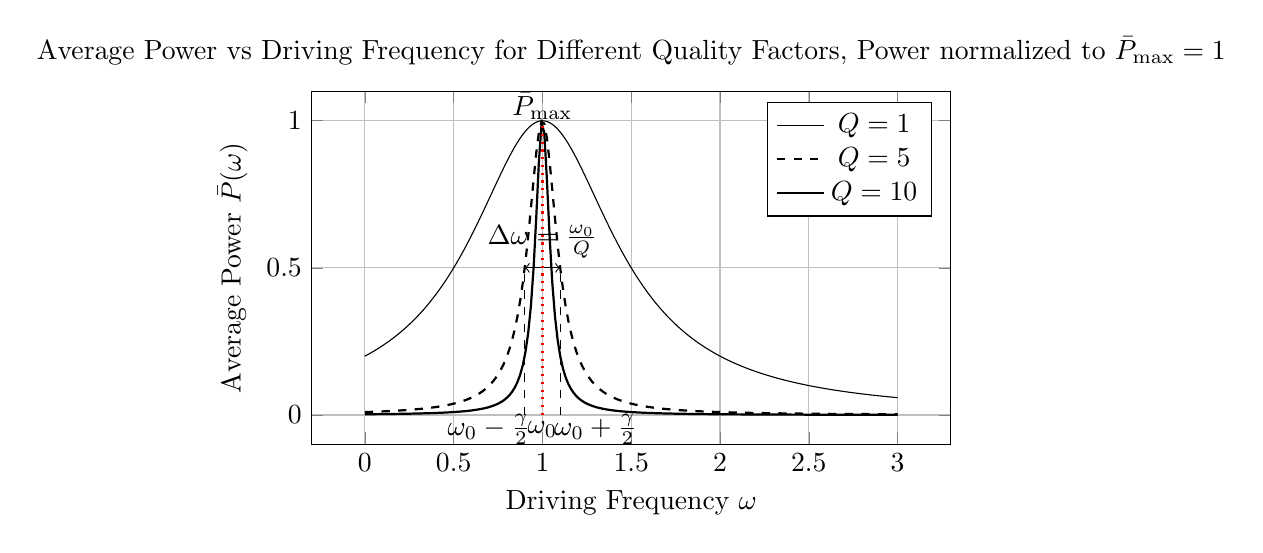
\begin{tikzpicture}
        \begin{axis}[
            xlabel={Driving Frequency \( \omega \)},
            ylabel={Average Power \( \bar{P}(\omega) \)},
            title={Average Power vs Driving Frequency for Different Quality Factors, Power normalized to \( \bar{P}_{\text{max}}  = 1\)},
            legend pos=north east,
            grid=major,
            width=0.8\textwidth,
            height=0.5\textwidth,
            domain=0:3,
            range=0:1.2,
            samples=200,
        ]
        % Plot for Q = 1
        \addplot[black] {1/(1 + (2*(x-1))^2)};
        \addlegendentry{\( Q = 1 \)}

        % Plot for Q = 5
        \addplot[black, thick, dashed] {1/(1 + (2*(x-1)/0.2)^2)};
        \addlegendentry{\( Q = 5 \)}

        % Plot for Q = 10
        \addplot[black, thick] {1/(1 + (2*(x-1)/0.1)^2)};
        \addlegendentry{\( Q = 10 \)}
        % add the lenght of the fwhm at P = 0.5
        \draw[dashed] (axis cs:0.9,0) -- (axis cs:0.9,0.5);
        \draw[dashed] (axis cs:1.1,0) -- (axis cs:1.1,0.5);
        \draw[<->] (axis cs:0.9,0.5) -- (axis cs:1.1,0.5) node[midway, above] {\( \Delta \omega = \frac{\omega_0}{Q} \)};
        
        % vertcal line dotted at omega = 1
        \draw[dotted, red, thick] (axis cs:1,0) -- (axis cs:1,1);
        % label the peak
        \node at (axis cs:1,1.05) {\( \bar{P}_{\text{max}} \)};
        % label the x axis at omega = 1
        \node at (axis cs:1,-0.05) {\( \omega_0 \)};
    
        % label the points
        \node at (axis cs:0.7,-0.05) {\( \omega_0 - \frac{\gamma}{2} \)};
        \node at (axis cs:1.3,-0.05) {\( \omega_0 + \frac{\gamma}{2} \)};
        
        \end{axis}
    \end{tikzpicture}
    \caption{Average Power vs Driving Frequency for Different Quality Factors}
    \label{fig:power_vs_frequency}
\end{figure}

\subsection{Simple Pendulum}

\begin{keybox}
\textbf{Key Equations:}
\begin{itemize}
    \item Small angle approximation: $\ddot{\theta} + \frac{g}{l}\theta = 0$ (valid for $\theta \ll 1$ rad)
    \item Period: $T = 2\pi\sqrt{l/g}$ (independent of mass!)
    \item Physical pendulum: $\omega = \sqrt{\frac{mgd}{I}}$ where $d$ is distance to CM
\end{itemize}
\textbf{Tip:} LC circuits are analogous to oscillators: $L \leftrightarrow m$, $1/C \leftrightarrow k$, $R \leftrightarrow b$
\end{keybox}

Consider the arc length \( s \) of a pendulum bob, we have:
$$
    s = l\theta \quad m\ddot{s} = -mg\sin(\theta)
$$

For small angles, we can approximate \( \sin(\theta) \approx \theta \), leading to:
$$
    \ddot{\theta} + \frac{g}{l}\theta = 0
$$
And the ODE has solution:
$$
    \theta(t) = \theta_0 \cos(\omega t + \phi)
$$

\paragraph{Energy} For small angle $\theta$, the total mechanical energy \( E \) of the pendulum is given by:
$$
    E = K + U = \frac{1}{2}ml^2\dot{\theta}^2 + mgl(1 - \cos(\theta)) \approx \frac{1}{2}ml^2\dot{\theta}^2 + \frac{1}{2}mgl\theta^2
$$
This shows that the pendulum behaves like a simple harmonic oscillator with an effective spring constant \( k = \frac{mg}{l} \).    


\paragraph{The physical pendulum} For a rigid body swinging about a pivot point, the equation of motion is given by:
$$
    I\ddot{\theta} = \tau 
$$
For simple rod of length \( L \) and mass \( m \) pivoted at one end, the moment of inertia about the pivot point is \( I = \frac{1}{3}mL^2 \). The torque due to gravity when the rod is displaced by an angle \( \theta \) from the vertical is \( \tau = -mg\frac{L}{2}\sin(\theta) \). For small angles, we can approximate \( \sin(\theta) \approx \theta \), leading to:
$$
    \ddot{\theta} + \frac{3g}{2L}\theta = 0
$$
And the small angle approximates leads to:
$$
    \ddot{\theta} + \omega^2 \theta = 0
$$
where \( \omega = \sqrt{\frac{3g}{2L}} \). The solution to this ODE is:
$$
    \theta(t) = \theta_0 \cos(\omega t + \phi)
$$
The angular frequency of oscillation for the physical pendulum is:
$$
    \omega = \sqrt{\frac{3g}{2L}}
$$

\paragraph{The LC Circuit} An LC circuit consists of an inductor \( L \) and a capacitor \( C \) connected in series. The charge \( q(t) \) on the capacitor satisfies the differential equation:
$$
    L\frac{d^2q}{dt^2} + \frac{1}{C}q = 0
$$
This is analogous to the equation of motion for a simple harmonic oscillator, with the angular frequency given by:
$$
    \omega = \frac{1}{\sqrt{LC}}
$$  

\paragraph{The RLC Circuit} An RLC circuit consists of a resistor \( R \), inductor \( L \), and capacitor \( C \) connected in series. The charge \( q(t) \) on the capacitor satisfies the differential equation:
$$
    L\frac{d^2q}{dt^2} + R\frac{dq}{dt} + \frac{1}{C}q = 0
$$
This is analogous to the resistor behaving as a damped harmonic oscillator, with the angular frequency given by:
$$
    \omega = \sqrt{\frac{1}{LC} - \left(\frac{R}{2L}\right)^2}
$$
The following are equations that summarize the analogies between mechanical and electrical oscillators:
\begin{table}[h!]
    \centering
    \begin{tabular}{|c|c|c|}
        \hline
        \textbf{Mechanical Oscillator} & \textbf{Electrical Oscillator} & \textbf{Analogy} \\
        \hline
        Mass \( m \) & Inductance \( L \) & Inertia \\
        Spring constant \( k \) & Inverse capacitance \( \frac{1}{C} \) & Restoring force \\
        Damping coefficient \( b \) & Resistance \( R \) & Energy dissipation \\
        Displacement \( x \) & Charge \( q \) & Position \\
        Velocity \( \dot{x} \) & Current \( I = \frac{dq}{dt} \) & Rate of change of position \\
        Force \( F \) & Voltage \( V \) & Driving force \\
        \hline
    \end{tabular}
    \caption{Analogies between Mechanical and Electrical Oscillators}
    \label{tab:oscillator_analogies}
\end{table}

\subsection{Coupled Oscillators}

\begin{keybox}
\textbf{Key Concepts:}
\begin{itemize}
    \item Normal coordinates $q_1 = x_1 + x_2$, $q_2 = x_1 - x_2$ decouple the equations
    \item Each normal mode has its own frequency: $\omega_1$ (in-phase), $\omega_2$ (out-of-phase)
    \item General motion = superposition of normal modes
    \item Energy doesn't flow between modes (they're independent)
\end{itemize}
\textbf{Tip:} Beat frequency $= (\omega_2 - \omega_1)/2$ describes energy transfer between oscillators!
\end{keybox}
\begin{definition}[Coupled Oscillators]
    Consider two masses \( m_1 \) and \( m_2 \) on two pendulum connected by springs with spring constant \( k \).  The equations of motion for the two masses are given by:

    $$
        \begin{cases}
            \ddot{x}_1 &= -\frac{g}{L}x_1 + \frac{k}{m_1} (x_1 - x_2) \quad (a) \\
            \ddot{x}_2 &= -\frac{g}{L}x_2 - \frac{k}{m_2} (x_1 - x_2) \quad (b)
        \end{cases}
    $$
    where \( x_1 \) and \( x_2 \) are the displacements of masses \( m_1 \) and \( m_2 \) from their equilibrium positions, respectively. Now if we add and subtract the two equations, we get:
    $$
        \begin{cases}
            \ddot{x}_1 + \ddot{x}_2 &= -\frac{g}{L}(x_1 + x_2) \quad (c) \\
            \ddot{x}_1 - \ddot{x}_2 &= -\left(\frac{g}{L} + \frac{k}{m_1} + \frac{k}{m_2}\right)(x_1 - x_2) \quad (d)
        \end{cases}
    $$
    Let:
    $$ 
    q_1 = x_1 + x_2 \quad \text{and} \quad q_2 = x_1 - x_2
    $$
    also, we let:
    $$
        \omega_1 = \sqrt{\frac{g}{L}} \quad \text{and} \quad \omega_2 = \sqrt{\frac{g}{L} + \frac{k}{m_1} + \frac{k}{m_2}}
    $$
    Then, the equations of motion can be rewritten as:
    $$
        \begin{cases}
            \ddot{q}_1 &= -\omega_1^2 q_1 \\
            \ddot{q}_2 &= -\omega_2^2 q_2
        \end{cases}
    $$
    Observe that \( q_1 \) and \( q_2 \) are decoupled, and each behaves like a simple harmonic oscillator with angular frequencies \( \omega_1 \) and \( \omega_2 \), respectively. The general solutions for \( q_1(t) \) and \( q_2(t) \) are:
    $$
        \begin{cases}
            q_1(t) &= A_1 \cos(\omega_1 t + \phi_1) \\
            q_2(t) &= A_2 \cos(\omega_2 t + \phi_2)
        \end{cases}
    $$
    where \( A_1, A_2, \phi_1, \) and \( \phi_2 \) are constants determined by the initial conditions. Finally, we can expressions for \( x_1(t) \) and \( x_2(t) \) in terms of \( q_1(t) \) and \( q_2(t) \):
    $$
        \begin{cases}
            x_1(t) &= \frac{q_1(t) + q_2(t)}{2} = \frac{A_1}{2} \cos(\omega_1 t + \phi_1) + \frac{A_2}{2} \cos(\omega_2 t + \phi_2) \\
            x_2(t) &= \frac{q_1(t) - q_2(t)}{2} = \frac{A_1}{2} \cos(\omega_1 t + \phi_1) - \frac{A_2}{2} \cos(\omega_2 t + \phi_2)
        \end{cases}
    $$
    All parts of the system oscillate with the same normal frequency (eigenvalue) in a normal mode (eigenvector).
\end{definition}

\begin{definition}[Normal Modes]
    A \textbf{normal mode} is a natural pattern of oscillation in which every part of the system moves in sync with a single frequency. 

    For the two-mass pendulum system, there are two normal modes:
    \begin{itemize}
        \item \textbf{In-phase mode} (\(\omega_1\)): both masses swing together, reaching maximum displacement on the same side at the same time.  
        $$
        x_1 = x_2
        $$
        
        \item \textbf{Out-of-phase mode} (\(\omega_2\)): the two masses swing in opposite directions, so when one moves left, the other moves right.  
        $$
        x_1 = -x_2
        $$
    \end{itemize}

    Any general motion of the system can be written as a combination (superposition) of these two normal modes.
\end{definition}
\paragraph{Energy in Coupled Oscillators} The total mechanical energy \( E \) of the coupled oscillator system is given by:
$$
    E = \frac{1}{2}m_1\dot{x}_1^2 + \frac{1}{2}m_2\dot{x}_2^2 + \frac{1}{2}k(x_1 - x_2)^2 + \frac{1}{2}m_1\frac{g}{L}x_1^2 + \frac{1}{2}m_2\frac{g}{L}x_2^2
$$
Substituting the expressions for \( x_1 = \frac{q_1 + q_2}{2} \) and \( x_2 = \frac{q_1 - q_2}{2} \) into the energy equation, two independent energies terms for $q_1$ and $q_2$ emerge:
$$
    E = \left[ \frac{1}{4} m \dot{q}_1^2 + \frac{1}{4}\frac{m_1 g}{L} q_1^2 \right] + \left[ \frac{1}{4} m \dot{q}_2^2 + \frac{1}{4}\frac{m_2 g}{L} q_2^2 \right]
$$
This shows that the total energy is the sum of the energies associated with each normal mode, and that no cross term between the modes exists. Thus energy does not flow from one mode to another.

\begin{example}
    Given two coupled pendulums with $x_0(0) = A$, $x_1(0) = 0$, and both masses at rest initially, we have:
    \begin{align*}
        q_0(t) &= C_0 \cos(\omega_0 t) \\
        q_1(t) &= C_1 \cos(\omega_1 t)
    \end{align*}
    where \( C_0 \) and \( C_1 \) are constants determined by the initial conditions. Using the initial conditions. Using the cosine addition formula, which is:
    \begin{align*}
        \cos(A) + \cos(B) &= 2\cos\left(\frac{A+B}{2}\right)\cos\left(\frac{A-B}{2}\right) \\
        \cos(A) - \cos(B) &= -2\sin\left(\frac{A+B}{2}\right)\sin\left(\frac{A-B}{2}\right)
    \end{align*}
    we can express the motion of each pendulum as:
    \begin{align*}
        x_0(t) &= \frac{q_0 + q_1}{2} = A \cos\left(\frac{\omega_0 + \omega_1}{2} t\right) \cos\left(\frac{\omega_0 - \omega_1}{2} t\right) \\
        x_1(t) &= \frac{q_0 - q_1}{2} = A \sin\left(\frac{\omega_0 + \omega_1}{2} t\right) \sin\left(\frac{\omega_0 - \omega_1}{2} t\right)
    \end{align*}
    Due to the formula for the product of cosines and sines, we see that energy oscillates between the two pendulums with a beat frequency of \( \frac{\omega_1 - \omega_0}{2} \). The time for all the energy to transfer from one pendulum to the other is given by:
    \begin{align*}
        T &= \frac{2\pi}{\frac{\omega_1 - \omega_0}{2}} = \frac{4\pi}{\omega_1 - \omega_0}
    \end{align*}

\end{example}
\subsection{Normal Modes}

\begin{keybox}
\textbf{Key Concepts:}
\begin{itemize}
    \item Normal mode = pattern where all parts oscillate at same frequency
    \item Find frequencies by solving eigenvalue problem: det$(K - \omega^2 M) = 0$
    \item Number of normal modes = number of degrees of freedom
    \item Eigenvectors give amplitude ratios for each mode
\end{itemize}
\textbf{Tip:} For symmetric systems, look for in-phase and out-of-phase modes!
\end{keybox}
\paragraph{Oscilating Masses Connected by Springs} Consider two masses \( m_1 = m_2 = m \) connected by three spring with spring constant \( k \) and fixed to walls on either side. The equations of motion for the two masses are given by:
$$
    \begin{cases}
        m\ddot{x}_1 &= -k x_1 + k (x_2 - x_1) \quad (a) = m\ddot{x}_1 = -2k x_1 + k x_2 \\
        m\ddot{x}_2 &= -k x_2 - k (x_2 - x_1) \quad (b) = m\ddot{x}_2 = k x_1 - 2k x_2
    \end{cases}
$$
To solve these equations, we assume solutions of the form:
$$
    \begin{cases}
        x_1(t) &= A \cos(\omega t + \phi) \\
        x_2(t) &= B \cos(\omega t + \phi)
    \end{cases}
$$
Substituting these assumed solutions into the equations of motion, we get:
\begin{equation} \label{eq:coupled_springs}
    \begin{cases}
        \frac{A}{B} &= \frac{k}{m\omega^2 - 2k} \\
        \frac{A}{B} &= \frac{m\omega^2 - 2k}{k}
    \end{cases}
\end{equation}
We can deduce that $A = \pm B$  
We can set the equation:
$$
    (m\omega^2 - 2k)^2 = k^2 \implies m\omega^2 - 2k = \pm k
$$

So we can derive two normal mode frequencies:
$$
    \begin{cases}
        \omega_1 &= \sqrt{\frac{k}{m}} \quad \text{(in-phase mode)} \\
        \omega_2 &= \sqrt{\frac{3k}{m}} \quad \text{(out-of-phase mode)}
    \end{cases}
$$

\paragraph{Solving as an Eigenproblem} Alternatively, we can create a system of equations from \eqref{eq:coupled_springs}:
$$
    \begin{bmatrix}
        \frac{2k}{m} & -\frac{k}{m} \\
        -\frac{k}{m} & \frac{2k}{m}
    \end{bmatrix}
    \begin{bmatrix}
        A \\ B
    \end{bmatrix}
    = \omega^2
    \begin{bmatrix}
        A \\ B
    \end{bmatrix}
$$
To find the eigenvalues \( \omega^2 \), we solve the characteristic equation:
$$
    \text{det}\left(\begin{bmatrix}
        \frac{2k}{m} - \omega^2 & -\frac{k}{m} \\
        -\frac{k}{m} & \frac{2k}{m} - \omega^2
    \end{bmatrix}\right) = 0
$$
Calculating the determinant, we have:
$$
    \left(\frac{2k}{m} - \omega^2\right)^2 - \left(-\frac{k}{m}\right)^2 = 0
$$
Expanding and simplifying, we get:
$$
    \omega^4 - \frac{4k}{m}\omega^2 + \frac{5k^2}{m^2} = 0
$$
This gives us the two normal mode frequencies:
$$
    \begin{cases}
        \omega_1^2 &= \frac{k}{m} \implies \omega_1 = \sqrt{\frac{k}{m}} \\
        \omega_2^2 &= \frac{3k}{m} \implies \omega_2 = \sqrt{\frac{3k}{m}}
    \end{cases}
$$

\begin{example}
    CConsider two equal masses $m$ suspended from identical springs of spring constant $k$. The masses are hanged on the celing. We can solve this system's frequency via the eigenvalue method. The equations of motion are:
    $$
        \begin{cases}
            m\ddot{x}_2 &= -k(x_2 - x_1)\\
            m\ddot{x}_1 &= -k x_1 + k(x_2 - x_1) = -2k x_1 + k x_2
        \end{cases}
    $$
    Assume solutions of the form:
    $$        
    \begin{cases}
            x_1(t) &= A \cos(\omega t + \phi) \\
            x_2(t) &= B \cos(\omega t + \phi)
        \end{cases}
    $$
    Substituting these assumed solutions into the equations of motion, we get:
    $$
        \begin{cases}
            -A \omega^2 &= -\frac{k}{m}(-2A + B) \\
            -B \omega^2 &= -\frac{k}{m}(A - B)
        \end{cases}
    $$
    We can rewrite this as an eigenvalue problem:
    $$
        \begin{bmatrix}
            \frac{2k}{m} & -\frac{k}{m} \\
            -\frac{k}{m} & \frac{k}{m}
        \end{bmatrix}
        \begin{bmatrix}
            A \\ B
        \end{bmatrix}
        = \omega^2
        \begin{bmatrix}
            A \\ B
        \end{bmatrix}
    $$
    To find the eigenvalues \( \omega^2 \), we solve the characteristic equation:
    $$
        \text{det}\left(\begin{bmatrix}
            \frac{2k}{m} - \omega^2 & -\frac{k}{m} \\
            -\frac{k}{m} & \frac{k}{m} - \omega^2
        \end{bmatrix}\right) = 0
    $$
    Calculating the determinant, we have:
    $$
        \omega^2 = \frac{k}{2m}(3\pm \sqrt{5})
    $$
\end{example}

\begin{example}
    Consider three equal masses \( m \) connected by four identical springs with spring constant \( k \) and fixed to walls on either side. The equations of motion for the three masses are given by:
    $$
        \begin{cases}
            m\ddot{x}_1 &= -2k x_1 + k x_2 \\
            m\ddot{x}_2 &= -2k x_2 + k x_1 + k x_3 \\
            m\ddot{x}_3 &= -2k x_3 + k x_2
        \end{cases}
    $$
    Assume solutions of the form:
    $$        
    \begin{cases}
            x_1(t) &= A \cos(\omega t + \phi) \\
            x_2(t) &= B \cos(\omega t + \phi) \\
            x_3(t) &= C \cos(\omega t + \phi)
        \end{cases}
    $$
    Substituting these assumed solutions into the equations of motion, we get:
    $$      
        \begin{cases}
            A \omega^2 &= -\frac{k}{m}(-2A + B) \\
            B \omega^2 &= -\frac{k}{m}(A - 2B + C) \\
            C \omega^2 &= -\frac{k}{m}(B - 2C)
        \end{cases}
    $$
    We can rewrite this as an eigenvalue problem:
    $$
        \begin{bmatrix}
            -\frac{2k}{m} & \frac{k}{m} & 0 \\
            \frac{k}{m} & -\frac{2k}{m} & \frac{k}{m} \\
            0 & \frac{k}{m} & -\frac{2k}{m}
        \end{bmatrix}
        \begin{bmatrix}
            A \\ B \\ C
        \end{bmatrix}
        = \omega^2
        \begin{bmatrix}
            A \\ B \\ C
        \end{bmatrix}
    $$
    To find the eigenvalues \( \omega^2 \), we solve the characteristic equation:
    $$
        \text{det}\left(\begin{bmatrix} 
            -\frac{2k}{m} - \omega^2 & \frac{k}{m} & 0 \\
            \frac{k}{m} & -\frac{2k}{m} - \omega^2 & \frac{k}{m} \\
            0 & \frac{k}{m} & -\frac{2k}{m} - \omega^2
        \end{bmatrix}\right) = 0
    $$
    Calculating the determinant, we have:
    $$        \left(\frac{2k}{m} - \omega^2\right)\left[\left(-\frac{2k}{m} - \omega^2\right)^2 - \left(\frac{k}{m}\right)^2\right] - \left(\frac{k}{m}\right)^2\left(\frac{2k}{m} - \omega^2\right) = 0
    $$   
    This gives us the three normal mode frequencies:
    $$
        \begin{cases}
            \omega_1 &= \sqrt{\frac{2k}{m}} \\
            \omega_2 &= \sqrt{\frac{2k}{m}(2 - \sqrt{2})} \\
            \omega_3 &= \sqrt{\frac{2k}{m}(2 + \sqrt{2})}
        \end{cases}
    $$
\end{example}
\paragraph{Intuition} For any perturbation, we can expressed it as a linear combination of the excitations of several normal modes. Each normal mode oscillates at its own frequency, and the overall motion is a superposition of these modes.
\section{Waves}

\subsection{Travelling Waves}

\begin{keybox}
\textbf{Key Equations:}
\begin{itemize}
    \item Wave function: $y(x,t) = A\cos(kx - \omega t + \phi_0)$ (travelling right)
    \item Wave speed: $v = \omega/k = f\lambda$
    \item Wave number: $k = 2\pi/\lambda$, Angular frequency: $\omega = 2\pi f$
    \item String wave speed: $v = \sqrt{\tau/\mu}$ where $\tau$ is tension, $\mu$ is linear density
\end{itemize}
\textbf{Common Pitfall:} Don't confuse particle velocity $(\partial y/\partial t)$ with wave velocity $v$!
\end{keybox}

\begin{definition}[Travelling Pulse]
    A travelling pulse is a disturbance that moves through a medium. For any wave function $f(x,t)$, if it satisfies the property:
    \begin{equation} \label{eq:travelling_wave}
        y(x,t) = f(x \pm vt)
    \end{equation}
    then it represents a wave travelling in the positive (for $x - vt$) or negative (for $x + vt$) x-direction with speed \( v \). $y$ could represent displacement, pressure, electric field, etc.
\end{definition}

\begin{definition}[Sinusoidal Wave]
    A sinusoidal wave is a wave that can be described by a sine or cosine function. The general form of a sinusoidal wave travelling in the positive x-direction is:
    $$
        y(x,t) = A \cos(kx \pm \omega t + \phi_0)
    $$
    where:
    \begin{itemize}
        \item \( A \) is the amplitude (maximum displacement)
        \item \( k = \frac{2\pi}{\lambda} \) is the wave number, with \( \lambda \) being the wavelength
        \item \( \omega = 2\pi f \) is the angular frequency, with \( f \) being the frequency
        \item \( \phi _0 \) is the initial phase.
    \end{itemize}
    So we can write the wave function as a form of \eqref{eq:travelling_wave}:
    $$
        y(x,t) = A \cos\left[k(x \pm vt) + \phi_0\right]
    $$
    The wave speed \( v \) is related to the angular frequency and wave number by:
    \begin{equation}\label{eq:wave_speed}
        v = \frac{\omega}{k} = f\lambda
    \end{equation}
\end{definition}

\paragraph{Transverse and Longitudinal Waves} There is two (or three) main categories of waves:
\begin{itemize}
    \item \textbf{Transverse Waves}: In transverse waves, the oscillations are perpendicular to the direction of wave propagation. \\
    (Examples) Light waves, water waves, and waves on a string.
    \item \textbf{Longitudinal Waves}: In longitudinal waves, the oscillations are parallel to the direction of wave propagation. \\
    (Examples) Sound waves and pressure waves in fluids.
    \item \textbf{Both}: Some waves can exhibit both transverse and longitudinal characteristics. \\
    (Examples) Rayleigh surface waves in seismology.
\end{itemize}
\begin{definition}[Velocity of a Fixed Particle]
    For a fixed particle, we have:
    $$
        v_y = \frac{\partial y}{\partial t} = A \omega \cos(kx \pm \omega t + \phi_0)
    $$
\end{definition}

\begin{example}[Vibrating String]
    Consider a string in the $xy$-plane, stretched along the x-axis with tension \( \tau \) and linear mass density \( \mu \). Now, consider at the end of the string at $x$ makes a small angle \( \theta \) with the x-axis. Then the components of the tension are:
    $$
    \begin{cases}
        \tau_x &= \tau \cos(\theta) \approx \tau \\
        \tau_y &= \tau \sin(\theta) \approx \tau \frac{\partial y}{\partial x}
    \end{cases}
    $$
    Now, consider a small segment of the string between \( x \) and \( x + \delta x \). The vetical force on the other end is given, via linear approximation, by:
    $$    
        \tau_y(x + \delta x) \approx \tau_y(x) \left[ \frac{\partial y}{\partial x}_x + \frac{\partial^2 y}{\partial x^2} \delta x \right]
    $$
    So the net force is given by:
    $$
        F_y = \tau_y(x + \delta x) - \tau_y(x) = \tau \frac{\partial^2 y}{\partial x^2} \delta x
    $$
    Because \( F=ma \), we have:
    $$
        \tau \frac{\partial^2 y}{\partial x^2} \delta x = \text{d}m \frac{\partial^2 y}{\partial t^2}
    $$
    where \( \text{d}m = \mu \delta x \) is the mass of the small segment. Thus, we have:
    $$
        \frac{\partial^2 y}{\partial t^2} - v^2 \frac{\partial^2 y}{\partial x^2} = 0
    $$
    where \( v = \sqrt{\frac{\tau}{\mu}} \) is the wave speed on the string. This is the one-dimensional wave equation.

\end{example}
\begin{definition}[The Wave Equation]
    The wave equation is a second-order linear partial differential equation that describes the propagation of waves (sound, EM, water) through a medium. In one dimension, it is given by:
    \begin{equation}\label{eq:wave_equation}
        \frac{\partial^2 u}{\partial t^2} - c^2 \frac{\partial^2 u}{\partial x^2} = 0
    \end{equation}
    where $u(x,t)$ is the disturbance, $c$ is the wave speed, $x$ is position, and $t$ is time.

    Or in general:
    $$
        \frac{\partial^2 u}{\partial t^2} - c^2 \nabla^2 u = 0
    $$
    where \( \nabla^2 \) is the Laplacian operator.
\end{definition}

\begin{definition}[Energy of a String]
    The kinetic energy of a string segment of mass \( \text{d}m = \mu \text{d}x \) is given by:
    $$
        \text{d}K = \frac{1}{2} \text{d}m v_y^2 = \frac{1}{2} \mu \text{d}x \left(\frac{\partial y}{\partial t}\right)^2
    $$
    The potential energy stored in the string due to its tension is given by:
    $$
        \text{d}U = \frac{1}{2} \tau (\delta s - \delta x) 
    $$
    where \( \delta s \) is the actual length of the string segment and \( \delta x \) is the horizontal length. For small displacements, we can approximate:
    $$
        \delta s \approx \delta x \left(1 + \frac{1}{2}\left(\frac{\partial y}{\partial x}\right)^2\right)
    $$
    Thus, the potential energy becomes:
    $$
        \text{d}U \approx \frac{1}{2} \tau \delta x \left(\frac{\partial y}{\partial x}\right)^2
    $$
    The total energy \( E \) of the string segment is the sum of its kinetic and potential energies:
    $$
        \text{d}E = \frac{1}{2} \mu \text{d}x \left(\frac{\partial y}{\partial t}\right)^2 + \frac{1}{2} \tau \text{d}x \left(\frac{\partial y}{\partial x}\right)^2
    $$
    For a sinusoidal wave \( y(x,t) = A \cos(kx - \omega t) \), the change in energy is:
    $$
        \text{d}E = \frac{1}{2} \mu A^2 \omega^2 \sin^2(kx - \omega t) \text{d}x + \frac{1}{2} \tau A^2 k^2 \sin^2(kx - \omega t) \text{d}x
    $$
    Integrating over one wavelength \( \lambda \), we find the total energy in one wavelength:
    $$
        E = \int_0^\lambda \text{d}E = \frac{1}{4} \mu A^2 \omega^2 \lambda + \frac{1}{4} \tau A^2 k^2 \lambda
    $$
    
\end{definition}

\begin{definition}[Power Transmitted by a String]
   The power carried by a transverse wave could be calculated from $P=Fv$. The transverse force on the string is given by:
    $$
        P(x,t) = A^2 \mu v \omega^2 \sin^2(kx - \omega t + \phi_0)
    $$
    The average power is then given by:
    $$
        \bar{P} = \frac{1}{2} A^2 \mu v \omega^2 = \frac{1}{2} \mu A^2 \omega^2 \frac{\lambda}{T}
    $$
    And the maximum power is given by:
    $$
        P_{max} = A^2 \mu v \omega^2
    $$
\end{definition}

\paragraph{Speed of Sound} The speed of sound waves through various meida is as follows:
\begin{itemize}
    \item In ideal gas, it is given by:
    $$
        v = \sqrt{\frac{\gamma RT}{m}} = \sqrt{\frac{\gamma k_B T}{m}}
    $$
    where \( \gamma \) is the adiabatic index, \( R \) is the universal gas constant, \( k_B \) is the Boltzmann constant, \( T \) is the absolute temperature, and \( m \) is the molar mass of the gas. $\gamma$ varies based on the type of gas:
    \begin{itemize}
        \item Monatomic gases (e.g., helium, neon): \( \gamma = \frac{5}{3} \)
        \item Diatomic gases (e.g., nitrogen, oxygen): \( \gamma = \frac{7}{5} \)
        \item Polyatomic gases (e.g., carbon dioxide, methane): \( \gamma \) is typically between 1.3 and 1.4
    \end{itemize}
    \item In a liquid, it is given by:
    $$
        v = \sqrt{\frac{B_{\text{adiabatic}}}{m}} = \sqrt{\frac{B}{\rho}}
    $$
    where \(B_{\text{adiabatic}}\) is the adiabatic bulk modulus, \( B \) is the bulk modulus, \( \rho \) is the density of the liquid and \( m \) is the molar mass of the liquid.
    \item In a solid, it is given by:
    $$
        v = \sqrt{\frac{E}{\rho}} 
    $$
    where \( E \) is the Young's modulus and \( \rho \) is the density of the solid. It could also be given by:
    $$
        v = \sqrt{\frac{B}{\rho}}
    $$
    where \( B \) is the bulk modulus.
\end{itemize}

\begin{definition}[Impedance]
    Similar to electrical impedance, we also have acoustic impedance and mechanical, they measure how much a structure recisits motion when subjected to a harmonic force. They are defined as follows:
    \begin{itemize}
        \item Electical impedance \( Z_e \):
        $$
            Z_e = \sqrt{R^2 + \left(\omega L - \frac{1}{\omega C}\right)^2}
        $$
        \item Acoustic impedance \( Z_a \), it is the ratio of acoustic pressure to particle velocity:
        $$
            Z_a = \frac{p}{v} = \rho v = \sqrt{B\rho}
        $$
        \item Mechanical impedance \( Z_m \):
        $$
            Z_m = v\mu = \sqrt{\tau\mu}
        $$
    \end{itemize}
\end{definition}

\paragraph{Wave boundry Conditions} When a wave encounters a boundary between two different media, part of the wave is reflected back into the original medium, and part is transmitted into the new medium. This is constrined by the following boundary conditions:
\begin{itemize}
    \item The displacement of the wave must be continuous across the boundary:
    $$
        y_1(x_b, t) = y_2(x_b, t) = y_3(x_b, t)
    $$
    \item The derivative of the displacement with respect to position must also be continuous across the boundary:
    $$
        \frac{\partial y_1}{\partial x}\bigg|_{x_b} = \frac{\partial y_2}{\partial x}\bigg|_{x_b} = \frac{\partial y_3}{\partial x}\bigg|_{x_b}
    $$
\end{itemize}
and then from these conditions, we can derive the amplitudes of the reflected and transmitted waves:
\begin{equation}\label{eq:amp-continuity}
    A_i = A_r + A_t
\end{equation}
and 
$$
    A_i Z_1 = A_r Z_1 + A_t Z_2
$$
From these two equations, we can solve for the reflection and transmission coefficients:
\begin{equation}\label{eq:reflection_coeff}
    R = \frac{A_r}{A_i} = \frac{Z_2 - Z_1}{Z_2 + Z_1}
\end{equation}
and
\begin{equation}\label{eq:transmission_coeff}
    T = \frac{A_t}{A_i} = \frac{2Z_2}{Z_2 + Z_1}
\end{equation}

\paragraph{Special Cases} There are two special cases:
\begin{itemize}
    \item \textbf{Fixed End}: If the wave encounters a boundary where the medium is fixed (e.g., a string tied to a wall), the reflected wave undergoes a phase change of \( \pi \) (inversion). The reflection coefficient is \( R = -1 \) and the transmission coefficient is \( T = 0 \).
    \item \textbf{Free End}: If the wave encounters a boundary where the medium is free to move (e.g., a string attached to a ring that can slide along a rod), the reflected wave does not undergo a phase change. The reflection coefficient is \( R = 1 \) and the transmission coefficient is \( T = 2 \).
\end{itemize}

\begin{example}[Transmission of 64\% Energy]
Suppose a wave transmits \(64\%\) of its incident energy across a boundary. Then:
$$
    T_e = 0.64, 
    \quad R_e = 1 - T_e = 0.36
$$
so that the amplitude reflection coefficient is
$$
    R = +\sqrt{R_e} = 0.6 
$$
\textbf{Important} the positive sign indicates the reflected wave is \emph{in phase} with the incident wave.

From the boundary condition in Eq.~\eqref{eq:amp-continuity},
$$
    T = 1 + R = 1 + 0.6 = 1.6
$$
Thus, the amplitude transmission coefficient is \(T = 1.6\), even though only \(64\%\) of the energy is transmitted. This apparent paradox arises because the transmitted energy depends on both the amplitude squared and the ratio of impedances \(\tfrac{Z_2}{Z_1}\).
\end{example}
\subsection{Superposition and Standing Waves}

\begin{keybox}
\textbf{Key Equations:}
\begin{itemize}
    \item Standing wave: $y(x,t) = 2A\sin(kx)\cos(\omega t)$ (for fixed-fixed ends)
    \item Allowed wavelengths: $\lambda_n = 2L/n$ where $n = 1,2,3,...$
    \item Frequencies: $f_n = nv/(2L) = nf_1$ (harmonics)
    \item Constructive interference: path difference $= m\lambda$
    \item Destructive interference: path difference $= (m+1/2)\lambda$
\end{itemize}
\textbf{Tip:} Nodes are spaced $\lambda/2$ apart; antinodes too!
\end{keybox}
\begin{definition}[Modulation of two waves]
    Consider two monochromatic waves:
    $$
    \begin{cases}
        y_1(x,t) &= A \cos(k_1 x - \omega_1 t) \\
        y_2(x,t) &= A \cos(k_2 x - \omega_2 t)
    \end{cases}
    $$
    Then, the resultant wave $y_1 + y_2$ can be expressed as:
    $$
        y(x,t) = 2A \cos\left(\frac{(k_1 - k_2)x - (\omega_1 - \omega_2)t}{2}\right) \cos\left(\frac{(k_1 + k_2)x - (\omega_1 + \omega_2)t}{2}\right)
    $$
\end{definition}

\begin{definition}[Coherence]
    Two waves are said to be coherent if they are monochromatic and maintain a constant phase relationship over time. This means that the difference in phase between the two waves does not change as they propagate:
    $$
        \Delta \phi = \phi_1 - \phi_2 = \text{constant}
    $$
    Coherent waves can produce stable interference patterns, such as constructive and destructive interference.
\end{definition}

\begin{definition}[Phase and Phase Difference]
    Phase of the wave is an argument $kx \pm \omega t + \phi_0$ of the wave function. The phase difference between two waves at a given point in space and time is given by:
    $$
        \Delta \phi = (k_1 x - \omega_1 t + \phi_1) - (k_2 x - \omega_2 t + \phi_2)
    $$
    where \( k_1, k_2 \) are the wave numbers, \( \omega_1, \omega_2 \) are the angular frequencies, and \( \phi_1, \phi_2 \) are the initial phases of the two waves.

    If we consider two waves of the same frequency and wave number, the phase difference simplifies to:
    $$
        \Delta \phi = \Delta\phi + k\Delta x + \omega \Delta t
    $$

\end{definition}
\begin{definition}[Waves in Two and Three Dimensions]
    In two or three dimensions, waves can propagate in various directions. The general form of a wave in two dimensions is:
    $$
        z(x,y,t) = A \cos(k_x x + k_y y - \omega t + \phi_0)
    $$
    where \( k_x \) and \( k_y \) are the wave numbers in the \( x \) and \( y \) directions, respectively, and \( \phi_0 \) is the initial phase. We also define $v$ and $k$ as:
    $$
        v = \frac{\omega}{k}, \quad k = \sqrt{k_x^2 + k_y^2}
    $$
\end{definition}

\begin{definition}[Spherical Waves]
    A spherical wave is a wave that propagates outward in all directions from a point source. The general form of a spherical wave is:
    $$
        y(r,t) = \frac{A}{r} \cos(kr - \omega t + \phi_0)
    $$
    where \( r = \sqrt{x^2 + y^2 + z^2} \) is the radial distance from the source, \( A \) is the amplitude at a reference distance, \( k \) is the wave number, \( \omega \) is the angular frequency, and \( \phi_0 \) is the initial phase. The amplitude decreases with distance as \( 1/r \) due to the spreading of the wavefront.
    
\end{definition}

\begin{definition}[Interference]
    Consider two coherent in phase sources $S_1$ and $S_2$ separated by a distance \( d \). The path difference \( \Delta r \) between the two waves at a point \( P \) is given by:
    $$
        \Delta r = r_2 - r_1
    $$
    where \( r_1 \) and \( r_2 \) are the distances from the sources \( S_1 \) and \( S_2 \) to the point \( P \), respectively.

    We have the following two cases for constructive and destructive interference:
    \begin{itemize}
        \item \textbf{Constructive Interference}: Occurs when the path difference is an integer multiple of the wavelength:
        $$
            \Delta r = m \lambda, \quad m = 0, 1, 2, \ldots
        $$
        \item \textbf{Destructive Interference}: Occurs when the path difference is an odd multiple of half the wavelength:
        $$
            \Delta r = \left(m + \frac{1}{2}\right) \lambda, \quad m = 0, 1, 2, \ldots
        $$
    \end{itemize}
\end{definition}

\paragraph{Nodes and Antinodes} In a standing wave, nodes are points where the medium does not move (zero displacement), while antinodes are points where the medium experiences maximum displacement. The distance between two consecutive nodes or antinodes is half the wavelength (\( \frac{\lambda}{2} \)). Nodes occur at positions where \( kx = n\pi \) (for integer \( n \)), and antinodes occur at positions where \( kx = (n + \frac{1}{2})\pi \).
\begin{definition}[Nodes]
    Nodes are points along a standing wave where the wave has zero amplitude. At these points, destructive interference occurs, and the medium remains at rest. Nodes occur at:
    $$
        x_n = n \frac{\lambda}{2}, \quad n = 0, 1, 2, \ldots
    $$
\end{definition}
\begin{definition}[Antinodes]
    Antinodes are points along a standing wave where the wave has maximum amplitude. At these points, constructive interference occurs, and the medium oscillates with the greatest displacement. Antinodes occur at:
    $$
        x_a = \left(n + \frac{1}{2}\right) \frac{\lambda}{2}, \quad n = 0, 1, 2, \ldots
    $$
\end{definition}

\paragraph{Antinodal Curves} In two-dimensional standing waves, antinodal curves are the loci of points where the amplitude of the wave is maximum. These curves are formed by the constructive interference of waves from multiple sources. The shape and spacing of antinodal curves depend on the geometry of the wave sources and the wavelength of the waves. An antindal curve could be visuallized as following:
\begin{figure}[h!]
    \centering
    % tikz, one source at (0, -3), another at (0, 3), cetner line at y = 0
    \resizebox{0.4\textwidth}{!}{
    
    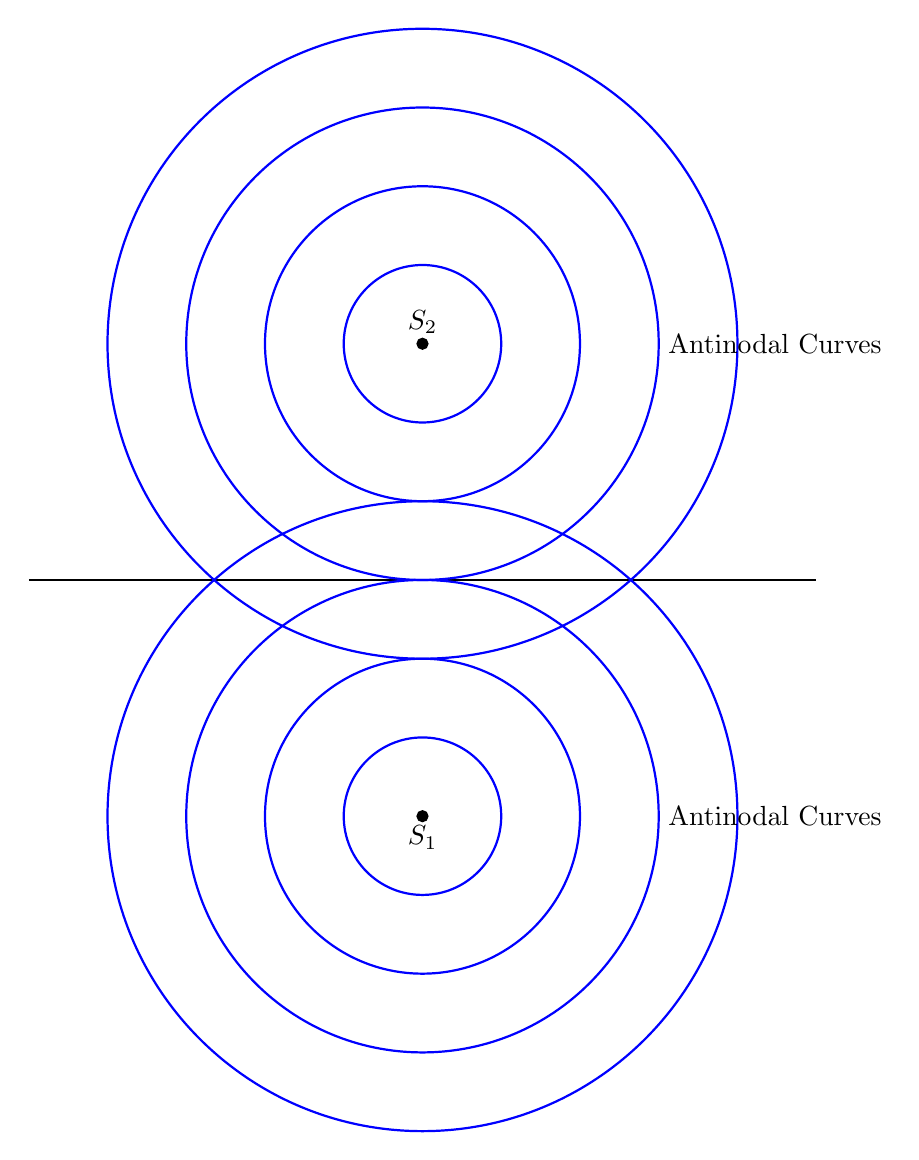
\begin{tikzpicture}
        % Draw the sources
        \filldraw[black] (0, -3) circle (2pt) node[below] {$S_1$};
        \filldraw[black] (0, 3) circle (2pt) node[above] {$S_2$};   
        % Draw the center line
        \draw[thick] (-5, 0) -- (5, 0) node[right] {};
        % Draw the antinodal curves as circles radiating from the sources
        \foreach \r in {1, 2, 3, 4} {
            \draw[blue, thick] (0, -3) circle (\r);
            \draw[blue, thick] (0, 3) circle (\r);
        }
        % Label the antinodal curves
        \node at (3, -3) [right] {Antinodal Curves};
        \node at (3, 3) [right] {Antinodal Curves};
    \end{tikzpicture}
    }
    \caption{Antinodal Curves}
    \label{fig:antinodal_curves}
\end{figure}


\begin{definition}[Standing Waves]
    Standing waves are formed by the superposition of two waves of the same frequency and amplitude traveling in opposite directions. The solution of the standing waves must satisfy a quantization condition, which leads to discrete frequencies and wavelengths. This discretized solution is given by:
    \begin{equation}\label{eq:standing_wave}
        y(x,t) = A_n \sin(kx) \cos(\omega t)
    \end{equation}
    where \( k = \frac{n\pi}{L} \) for \( n = 1, 2, 3, \ldots \), and \( L \) is the length of the medium (e.g., a string fixed at both ends). The corresponding frequencies are given by: 
    $$
        f_n = \frac{n v}{2L}
    $$
    In turn, the wavelengths are given by:
    $$
        \lambda_n = \frac{2L}{n}
    $$
    where \( v \) is the wave speed. The distance between two consecutive nodes or antinodes is given by:
    $$
        d = \frac{\lambda}{2}
    $$
    
\end{definition}

\paragraph{Systems with no Fixed Ends} For systems with no fixed ends, the general solution is given by:
$$
    y(x,t) = A_n \cos(kx) \cos(\omega_n t)
$$
where \( k = \frac{n\pi}{L} \) for \( n = 0, 1, 2, \ldots \). 
the postion of the nodes are:
$$
    x_n = n \frac{\lambda}{2}, \quad n = 0, \pm 1, \pm 2, \ldots
$$
and the position of the antinodes are:
$$
    x_a = \left(n + \frac{1}{2}\right) \frac{\lambda}{2}, \quad n = 0, \pm 1, \pm 2, \ldots
$$

\paragraph{Systems with no free Ends} For systems with no free ends, the general solution is given by:
$$
    y(x,t) = A_n \sin(kx) \cos(\omega_n t)
$$

The postion of the nodes are:
$$
    x_n = \left(n + \frac{1}{2}\right) \frac{\lambda}{2}, \quad n = 0, 1, 2, \ldots
$$
and the position of the antinodes are:
$$
    x_a = n \frac{\lambda}{2}, \quad n = 0, 1, 2, \ldots
$$

\paragraph{System with Mixed Ends} For systems with mixed ends (one fixed and one free), the general solution has two cases:
$$
    y(x,t) = \begin{cases}
        A_n \sin(kx) \cos(\omega_n t) & \text{if the fixed end is at } x=0 \\
        A_n \cos(kx) \cos(\omega_n t) & \text{if the fixed end is at } x=L
    \end{cases}
$$
The postion of the nodes are:
$$
    x_n = \left(n + \frac{1}{2}\right) \frac{\lambda}{2}, \quad n = 0, 1, 2, \ldots
$$
and the position of the antinodes are:
$$
    x_a = n \frac{\lambda}{2}, \quad n = 0, 1, 2, \ldots
$$

\begin{definition}[Energy of Standing Waves]
    The total energy stored in a standing wave on a string of length \( L \) is given by:
    $$
        E = \frac{1}{4} \mu A^2 \omega^2 L
    $$
    where \( \mu \) is the linear mass density of the string, \( A \) is the amplitude of the wave, and \( \omega \) is the angular frequency. The energy is equally divided between kinetic and potential energy, with each contributing half of the total energy.
\end{definition}

\begin{definition}[Average Power of Standing Waves]
    The average power transmitted by a standing wave on a string is given by:
    $$
        \bar{P} = \frac{1}{2} \mu A^2 \omega^2 v
    $$
    where \( \mu \) is the linear mass density of the string, \( A \) is the amplitude of the wave, \( \omega \) is the angular frequency, and \( v \) is the wave speed. This power represents the rate at which energy is transferred along the string.
    
\end{definition}
\subsection{Fourier analysis}
\begin{definition}[Standing Waves as Normal Modes of a Vibrating String]
    The superposition principle states that if $y_1(x,t)$ and $y_2(x,t)$ are two solutions to the wave equation, then their sum $y(x,t) = y_1(x,t) + y_2(x,t)$ is also a solution. For a string fixed at both ends, the $n^\text{th}$ normal mode of vibration can be expressed as:
    \begin{equation}
        y_n(x,t) = A_n \sin\left(\frac{n\pi x}{L}\right) \cos(\omega_n t)
    \end{equation}
    
    The motion of the string will be a superposition of normal modes:
    \begin{equation}
        y(x,t) = \sum_{n=1}^{\infty} A_n \sin\left(\frac{n\pi x}{L}\right) \cos(\omega_n t)
    \end{equation}
    where \( A_n \) are the amplitudes of the respective modes, and \( \omega_n = \frac{n\pi v}{L} \) are the angular frequencies of the modes.
\end{definition}

\begin{definition}[The amplitude of normal modes – Fourier analysis]
    If we look at the initial shape of the string:
    $$
        y(x,0) = \sum_n A_n \sin\left(\frac{n\pi x}{L}\right)
    $$
    Any initial shape of the string can be expressed as a Fourier sine series. Also, for fixed ends ($f(0)=f(L)=0$), we can write the shape as the following:
    $$
        f(x) = \sum_n A_n \sin\left(\frac{n\pi x}{L}\right)
    $$


    To find the coefficients \( A_n \), we use:
    \begin{equation}
        A_n = \frac{2}{L} \int_0^L f(x) \sin\left(\frac{n\pi x}{L}\right) \, dx
    \end{equation}
\end{definition}

\chapter{Modern Physics}
\section{Quantum Mechanics}
\begin{definition}[Quantization]
    Quantization is the constraint that energy and other physical properties can only take on discrete values (\textit{quanta}) rather than a continuous range.
\end{definition}
\begin{definition}[Probabilistic Framework]
    Predictions in quantum mechanics are inherently probabilistic. The exact outcome of a measurement cannot be determined, only the probability of different outcomes.
\end{definition}


\begin{definition}[Black Body]
    A black body is an idealized physical object that absorbs all incident electromagnetic radiation, regardless of frequency or angle of incidence. It also emits radiation in a characteristic spectrum that depends solely on its temperature.
\end{definition}
\begin{definition}[Classical View of Black Body Radiation]
    According to classical physics, Reyleigh-Jeans law predicts that the energy density of black body radiation increases indefinitely with frequency, leading to the "ultraviolet catastrophe." The classical formula is given by:
    $$    u(\nu, T) = \frac{8\pi \nu^2 k_B T}{c^3} $$
    where \( u(\nu, T) \) is the energy density per unit frequency, \( \nu \) is the frequency, \( k_B \) is the Boltzmann constant, \( T \) is the absolute temperature, and \( c \) is the speed of light.
\end{definition}
\begin{definition}[Quantum View of Black Body Radiation]
    Max Planck resolved the ultraviolet catastrophe by proposing that electromagnetic energy is quantized. He introduced the concept that energy is emitted or absorbed in discrete packets called \textbf{quanta}, with energy given by:
    \begin{equation}
        E_n = n h f \quad n = 0, 1, 2, \ldots
    \end{equation}
    where \( h \) is Planck's constant and \( f \) is the frequency of the radiation. This leads to Planck's law for black body radiation. The resulting law for the black body spectrum is:
    \begin{equation}
        u(\nu, T) = \frac{8\pi h \nu^3}{c^3} \frac{1}{e^{\frac{h\nu}{k_B T}} - 1}
    \end{equation}
\end{definition}



\begin{definition}[Photoelectric Effect]
    The photoelectric effect is the phenomenon where electrons are emitted from a material (usually a metal) when it is exposed to light of sufficient frequency. The key observations of the photoelectric effect are:
    \begin{itemize}
        \item Electrons are emitted only if the incident light has a frequency above a certain threshold frequency \( f_0 \).
        \item The kinetic energy of the emitted electrons depends on the frequency of the incident light, not its intensity.
        \item The number of emitted electrons is proportional to the intensity of the incident light, provided the frequency is above the threshold.
    \end{itemize}
    The energy of the incident photons is given by:
    $$
        E = h f
    $$
    where \( h \) is Planck's constant and \( f \) is the frequency of the light. The maximum kinetic energy \( K_{max} \) of the emitted electrons is given by:
    $$
        K_{max} = h f - \phi
    $$
    where \( \phi \) is the work function of the material, representing the minimum energy required to liberate an electron from the surface.
    
\end{definition}

\begin{definition}[Campton Effect]
    The Compton effect is the increase in wavelength (or decrease in energy) of X-rays or gamma rays when they are scattered by electrons. This phenomenon provides evidence for the particle-like behavior of light. The change in wavelength \( \Delta \lambda \) of the scattered photon is given by the Compton formula:
    \begin{equation}
        \Delta \lambda = \lambda' - \lambda = \frac{h}{m_e c} (1 - \cos \theta)
    \end{equation}
    where:
    \begin{itemize}
        \item \( \lambda \) is the initial wavelength of the photon,
        \item \( \lambda' \) is the wavelength after scattering,
        \item \( h \) is Planck's constant,
        \item \( m_e \) is the rest mass of the electron,
        \item \( c \) is the speed of light,
        \item \( \theta \) is the angle at which the photon is scattered.
    \end{itemize}
    
\end{definition}
\end{document}

